% Reporte de métricas: MongoDB frente a PostgreSQL JSONB bajo contención (cgroups v2).
% Compilar desde report/:  pdflatex reporte.tex  (dos veces, por las referencias)
% Las tablas de report/tablas/ y las figuras de report/figures/ las genera
% scripts/analyze_results.py a partir de results/.
\documentclass[11pt,letterpaper]{article}

\usepackage[utf8]{inputenc}
\usepackage[T1]{fontenc}
% es-noshorthands: sin él, babel convierte < y > en atajos y rompe el código como data->>'campo'.
\usepackage[spanish,es-tabla,es-nodecimaldot,es-noshorthands]{babel}
\usepackage{amsmath}
\usepackage{lmodern}
\usepackage[margin=2.2cm]{geometry}
\usepackage{graphicx}
\usepackage{booktabs}
\usepackage{array}
\usepackage{tabularx}
\usepackage{float}
\usepackage{caption}
\usepackage{xcolor}
\usepackage{enumitem}
\usepackage{listings}
\usepackage[hidelinks]{hyperref}

\graphicspath{{figures/}}
\captionsetup{font=small,labelfont=bf}
\setlist{itemsep=2pt,topsep=4pt}
% Permite estirar el espacio entre palabras antes que sacar del margen rutas y nombres largos.
\setlength{\emergencystretch}{3em}
\lstset{basicstyle=\ttfamily\footnotesize,breaklines=true,frame=single,columns=fullflexible}

\newcommand{\tablaperfil}[1]{%
    \begin{table}[H]\centering\scriptsize\setlength{\tabcolsep}{3.5pt}
    \caption{Resultados consolidados del perfil #1: mediana de 3 repeticiones. Latencias en
    segundos; throttling y RSS máximo de la ventana de medición de 300\,s.}
    \label{tab:res#1}
    \input{tablas/resultados_#1.tex}
    \end{table}}

\hypersetup{
  pdftitle={Medición de métricas en bases documentales},
  pdfauthor={Luis Ángel Pérez Aguilera}}

\begin{document}

\hypersetup{pageanchor=false}
\begin{titlepage}
\centering
{\LARGE\bfseries Universidad Politécnica de Chiapas\par}
\vspace{0.6cm}
{\large Ingeniería en Tecnologías de la Información e Innovación Digital\par}
\vspace{0.3cm}
{\large Bases de Datos en la Nube\par}

\vfill
\rule{\linewidth}{0.6pt}\par\vspace{0.5cm}
{\huge\bfseries Medición de métricas en bases documentales\par}
\vspace{0.4cm}
{\Large MongoDB frente a PostgreSQL JSONB bajo contención de CPU y memoria (Docker cgroups~v2)\par}
\vspace{0.5cm}\rule{\linewidth}{0.6pt}\par
\vfill

\begin{tabular}{rl}
\textbf{Alumno:}  & Luis Ángel Pérez Aguilera \\[4pt]
\textbf{Grupo:}   & 7B \\[4pt]
\textbf{Docente:} & Horacio Irán Solís Cisneros \\
\end{tabular}

\vfill
{\large 1 de noviembre de 2026\par}
\end{titlepage}
\hypersetup{pageanchor=true}

\begin{abstract}
\noindent Se comparan MongoDB~9.0.4 y PostgreSQL~18.6 (JSONB) al ejecutar dos agregaciones sobre
500\,000 documentos JSON con tres niveles de anidamiento, bajo tres perfiles de recursos impuestos
con cgroups~v2: A (4~CPU / 4\,GB), B (2~CPU / 2\,GB) y C (1~CPU / 1\,GB). Cada celda de la matriz
(2 motores $\times$ 3 perfiles $\times$ 2 consultas $\times$ 3 concurrencias, más las dos
variantes de memoria de Q2) se midió tres veces con el ciclo
\emph{flush} $\rightarrow$ warmup 60\,s $\rightarrow$ medición 300\,s $\rightarrow$ cooldown 60\,s:
162 corridas en total. La agregación con desanidado (Q1) separa a los motores: MongoDB la
resuelve en flujo con $\sim$128\,KB de memoria de agrupación y queda limitada solo por CPU, mientras
que PostgreSQL ordena filas completas con \emph{external merge}, escribe del orden de 1\,GB
temporal por consulta y, con 1\,GB y 50 clientes, termina en OOM. El Top-1000 (Q2) no produce
spill en ningún motor ni variante: ambos lo resuelven con un ordenamiento top-$k$ de menos de
1,1\,MB, y el límite de CPU domina su latencia.
\end{abstract}

\tableofcontents
\newpage

% =============================================================================
\section{Especificaciones del host y del entorno Docker}
\label{sec:host}

\subsection{Equipos}
Para completar la matriz en una sola jornada, las mediciones se repartieron en dos rondas
simultáneas en dos equipos. La ronda~1 midió los perfiles A y C \emph{en paralelo}
en el equipo principal; la ronda~2 midió el perfil B en un segundo equipo. De este modo el baseline (A) y
la contención severa (C) comparten hardware, y solo B se midió en otro equipo
(sección~\ref{sec:validez}).

\begin{table}[H]\centering\small
\caption{Equipos de medición (datos de \texttt{results/entorno/ronda*/host.txt}).}
\label{tab:host}
\begin{tabularx}{\linewidth}{l>{\raggedright\arraybackslash}X>{\raggedright\arraybackslash}X}
\toprule
 & Ronda 1 (perfiles A y C) & Ronda 2 (perfil B) \\
\midrule
CPU & Intel Core i5-13420H, 8 núcleos / 12 hilos & Dell Vostro 3400, Intel Core i5-1135G7 @ 2.40\,GHz, 4 núcleos / 8 hilos \\
RAM del equipo & 16\,GB (15.7\,GB útiles) & 8\,GB \\
Sistema & Windows 11 + WSL2 (Ubuntu 24.04), kernel 6.6.87.2-microsoft-standard-WSL2 & Windows 11 + WSL2 (Ubuntu), kernel 6.18.54.1-microsoft-standard-WSL2 \\
Memoria de la VM WSL2 & 7.6\,GB (valor por defecto) + 2\,GB de swap & 4.8\,GB (\texttt{.wslconfig}) + 2\,GB de swap \\
Docker & Docker Desktop, Engine 29.7.2, cgroup~v2 & Docker Desktop, Engine 29.9.2, cgroup~v2 (driver \texttt{cgroupfs}) \\
\bottomrule
\end{tabularx}
\end{table}

\subsection{Motores, imágenes y configuración}
\begin{itemize}
  \item \textbf{MongoDB 9.0.4} (\texttt{mongo:9.0.4}, digest \texttt{sha256:452bdaf2\ldots}),
        motor WiredTiger, colección \texttt{resultados\_unidad} sin sharding, índices simples en
        \texttt{resultado\_id} y \texttt{cerrado\_en}.
  \item \textbf{PostgreSQL 18.6} (\texttt{postgres:18.6}, digest \texttt{sha256:3a426452\ldots}),
        tabla \texttt{resultados\_unidad (id UUID PRIMARY KEY, data JSONB)}, PK en \texttt{id} y
        B-Tree sobre la expresión \texttt{data->>'cerrado\_en'}.
  \item Ninguno de los dos índices cubre el total del Top-K (\texttt{calificacion.final}), como
        exige la especificación.
  \item Configuración \textbf{por defecto} en ambos motores. WiredTiger dimensiona su caché
        a partir del límite de memoria del contenedor. PostgreSQL usa \texttt{shared\_buffers} y
        \texttt{work\_mem} (4\,MB) por defecto y hasta 2 workers paralelos por consulta. Lo único
        que se cambia es \texttt{work\_mem} por sesión en las variantes de Q2.
  \item Telemetría: cAdvisor v0.53.0, Node Exporter v1.9.1 y Prometheus v3.5.0 con
        \texttt{scrape\_interval: 1s}, fuera de los límites de los contenedores medidos.
\end{itemize}

\subsection{Perfiles de recursos y límites reales verificados}
Los perfiles se declaran en \texttt{infra/docker-compose.yml} con \texttt{cpus},
\texttt{mem\_limit}, \texttt{mem\_swappiness: 0} y \texttt{memswap\_limit}. En cgroup~v2 la
\emph{swappiness} por contenedor no existe y Docker la descarta, así que además se iguala
\texttt{memswap\_limit} a \texttt{mem\_limit}, lo que deja el swap del contenedor en cero.
Antes de cada bloque de corridas, el programa de medición registra los límites efectivos
leídos de la propia cgroup (\texttt{results/entorno/ronda*/<perfil>\_<motor>.txt}):

\begin{table}[H]\centering\small
\caption{Límites declarados y valores leídos de la cgroup~v2 de cada contenedor.}
\label{tab:limites}
\begin{tabular}{llllll}
\toprule
Perfil & \texttt{cpus} & \texttt{mem\_limit} & \texttt{cpu.max} & \texttt{memory.max} & \texttt{memory.swap.max} \\
\midrule
A \texttt{PROFILE\_A\_BASELINE} & 4.0 & 4096\,MB & \texttt{400000 100000} & 4\,294\,967\,296 & 0 \\
B \texttt{PROFILE\_B\_MEDIUM}   & 2.0 & 2048\,MB & \texttt{200000 100000} & 2\,147\,483\,648 & 0 \\
C \texttt{PROFILE\_C\_SEVERE}   & 1.0 & 1024\,MB & \texttt{100000 100000} & 1\,073\,741\,824 & 0 \\
\bottomrule
\end{tabular}
\end{table}

\noindent Cada perfil tiene su propio par de contenedores (MongoDB y PostgreSQL) con sus
propios volúmenes de datos. Durante una corrida solo está encendido el motor que se mide, para que
la caché del motor inactivo no ocupe memoria del equipo.

% =============================================================================
\section{Método de medición y verificación del baseline}
\label{sec:metodo}

\subsection{Dataset}
El esquema de ejemplo de la especificación de la actividad (órdenes de compra) se sustituyó por la colección
\texttt{resultados\_unidad} de un proyecto de control académico, conservando lo que
exige la especificación: 500\,000 documentos JSON, tres niveles de anidamiento
(\texttt{contexto.materia.nombre}, \texttt{calificacion.desglose[].criterio}), un arreglo de
2 a 4 elementos (promedio 3.0), un identificador UUID y una fecha ISO-8601 en formato UTC fijo.
El generador (\texttt{data/synthetic\_data\_generator.py}) es determinista (semilla 42); el
NDJSON resultante tiene sha256 \texttt{10a04043\ldots c429} y se carga idéntico en los dos motores.
La tabla~\ref{tab:mapeo} muestra qué campo cumple cada papel de las consultas de la
especificación.

\begin{table}[H]\centering\footnotesize
\caption{Campos de la especificación y campos equivalentes del dataset usado.}
\label{tab:mapeo}
\begin{tabular}{lll}
\toprule
Papel en la consulta & Campo en la especificación & Campo usado \\
\midrule
Arreglo que se desanida (Q1) & \texttt{items[]} & \texttt{calificacion.desglose[]} \\
Filtro numérico (Q1) & \texttt{price > 50} & \texttt{desglose.promedio > 6} \\
Subtotal (Q1) & \texttt{qty * price} & \texttt{porcentaje * promedio} \\
Claves de agrupación (Q1) & país, categoría & \texttt{contexto.materia.nombre}, \texttt{desglose.criterio} \\
Estado (Q2) & \texttt{payment.status = completed} & \texttt{unidad.estado = 'cerrada'} \\
Fecha (Q2) & \texttt{timestamp >= 2026-01-01} & \texttt{cerrado\_en >= 2026-01-01T00:00:00Z} \\
Total del Top-K (Q2) & \texttt{payment.final\_total} & \texttt{calificacion.final} \\
\bottomrule
\end{tabular}
\end{table}

\subsection{Consultas}
Q1 desanida el desglose (1\,500\,160 elementos), filtra los promedios mayores que 6
(974\,583 elementos) y agrupa en 180 grupos con suma, promedio y conteo. Q2 filtra las unidades
cerradas desde 2026 (212\,641 documentos), ordena de forma descendente por la calificación final
sin índice y devuelve el Top-1000. El código está en \texttt{queries/}; la versión de PostgreSQL:

\begin{lstlisting}[language=SQL]
-- Q1
SELECT data->'contexto'->'materia'->>'nombre' AS materia, d->>'criterio' AS criterio,
       SUM((d->>'porcentaje')::numeric * (d->>'promedio')::numeric) AS total_aporte,
       AVG((d->>'porcentaje')::numeric * (d->>'promedio')::numeric) AS avg_aporte,
       COUNT(*) AS count
FROM resultados_unidad, jsonb_array_elements(data->'calificacion'->'desglose') AS d
WHERE (d->>'promedio')::numeric > 6
GROUP BY 1, 2;
-- Q2
SELECT data->>'resultado_id', data->'alumno'->>'id', (data->'calificacion'->>'final')::numeric
FROM resultados_unidad
WHERE data->'unidad'->>'estado' = 'cerrada' AND data->>'cerrado_en' >= '2026-01-01T00:00:00Z'
ORDER BY (data->'calificacion'->>'final')::numeric DESC
LIMIT 1000;
\end{lstlisting}

\noindent La fecha se compara como texto: el cast a \texttt{timestamptz} de la especificación no es
inmutable y anula el índice de expresión; con el formato UTC fijo el orden del texto es el
cronológico y coincide con la comparación de cadenas de MongoDB. Las variantes de memoria de Q2 se
codifican en \texttt{query\_id} para no agregar columnas al CSV: \texttt{Q2\_DISK0} /
\texttt{Q2\_DISK1} (\texttt{allowDiskUse} false / true) en MongoDB y \texttt{Q2\_WM4} /
\texttt{Q2\_WM64} (\texttt{work\_mem} 4\,MB / 64\,MB) en PostgreSQL.

\subsection{Protocolo}
\begin{itemize}
  \item \textbf{Matriz.} Una \emph{celda} es una combinación de motor, perfil, consulta y
        concurrencia; cada celda se mide 3 veces y cada medición es una \emph{corrida}.
        2 motores $\times$ 3 perfiles $\times$ (Q1 + 2 variantes de Q2) $\times$ concurrencias
        1, 10 y 50 $\times$ 3 repeticiones = 162 corridas (54 por perfil), cada una con una fila
        en el CSV de 14 columnas que fija la especificación.
  \item \textbf{Ciclo por corrida.} \texttt{sync; echo 3 > /proc/sys/vm/drop\_caches}, warmup de
        60\,s, medición de 300\,s y cooldown de 60\,s. El flush se ejecuta en un contenedor
        privilegiado, que comparte el kernel de la VM. Cada corrida duró 423--424\,s
        según los registros de ejecución (\texttt{results/logs/}).
  \item \textbf{Perfiles en paralelo.} Como el flush de caché afecta a todo el kernel, las
        mediciones de A y C, que corrieron al mismo tiempo en el mismo equipo, se sincronizan
        antes de cada corrida: cada una espera a la otra, solo una ejecuta el flush y ambas
        arrancan en el mismo segundo. Así ninguna vacía la caché a la otra a mitad de una
        medición.
  \item \textbf{Programa de medición} (\emph{runner}, carpeta \texttt{runner/}, en Python).
        Usa un proceso por perfil y simula cada cliente concurrente con un hilo que tiene su
        propia conexión (pymongo 4.19, psycopg 3.3) y lanza una consulta tras otra sin pausa. Es
        una desviación menor del ``Python multiproceso'' de la especificación: los drivers
        liberan el GIL mientras esperan a la base de datos, y el programa usa $\sim$150\,MB por
        perfil en lugar de 1--2\,GB con 50 procesos.
  \item \textbf{Ventana de medición}. Cada consulta recibe como \emph{timeout} el tiempo
        que le queda a la ventana (\texttt{maxTimeMS} / \texttt{statement\_timeout}). Latencias y
        throughput cuentan solo las consultas que empiezan y terminan dentro de los 300\,s.
\end{itemize}

\subsection{Métricas y estado de cada corrida}
\begin{itemize}
  \item \textbf{Latencia}: percentiles P50, P95 y P99 de las latencias individuales (no promedios);
        las latencias crudas de cada corrida están en \texttt{results/raw/}.
  \item \textbf{Throughput}: consultas terminadas $\div$ 300\,s.
  \item \textbf{Throttling}: tiempo que el kernel detuvo al contenedor por haber agotado su
        \emph{cuota} de CPU (el límite \texttt{cpus} del perfil). Es el delta de
        \texttt{throttled\_usec} de \texttt{cpu.stat}, la misma métrica que
        \texttt{container\_cpu\_cfs\_throttled\_seconds\_total}. Puede superar los 300\,s de la
        ventana porque el kernel suma el tiempo de cada CPU donde había hilos del contenedor
        esperando.
  \item \textbf{CPU-s}: segundos de CPU consumidos por el contenedor en la ventana. Con la cuota
        agotada equivalen a CPUs del perfil $\times$ 300\,s (1\,200 en A, 600 en B, 300 en C).
  \item \textbf{RSS máximo}: máximo de \texttt{container\_memory\_rss} (memoria anónima) en la
        ventana. En PostgreSQL no incluye los buffers compartidos.
  \item \textbf{Spill}: delta de \texttt{pg\_stat\_database.temp\_bytes} en PostgreSQL y de los
        contadores de spill de \texttt{serverStatus} en MongoDB.
  \item \textbf{OOM}: delta de \texttt{oom\_kill} en \texttt{memory.events} del contenedor.
  \item \textbf{Estado}: \texttt{oom} si hubo OOM; \texttt{error} si hubo fallos o ninguna
        consulta terminó en la ventana; \texttt{spill} si hubo volcado a disco; \texttt{ok} en
        otro caso. Las corridas \texttt{spill}, \texttt{oom} o con fallos guardan evidencia
        (notas, \texttt{memory.events} y log del motor) en \texttt{results/evidencia\_spill\_oom/}.
\end{itemize}

\subsection{Resumen de repeticiones}
Cada celda se resume con la \textbf{mediana} de sus 3 repeticiones y el mínimo y máximo como rango:
con tres valores, una corrida atípica desplaza mucho la media. El consolidado completo está
en \texttt{report/datos/consolidado.csv} y lo genera \texttt{scripts/analyze\_results.py}.

\subsection{Verificación del baseline}
\begin{itemize}
  \item \textbf{Mismo dataset en todos los perfiles}: conteo de 500\,000 en ambos motores, índices
        exigidos y muestra de 25 documentos idéntica en MongoDB, PostgreSQL y el NDJSON
        (\texttt{scripts/validate\_data.py}).
  \item \textbf{Mismas consultas}: Q1 y Q2 devuelven el mismo resultado en ambos motores
        (\texttt{scripts/check\_queries.py}); en Q1 las sumas se comparan con tolerancia relativa
        de $10^{-9}$ porque MongoDB suma en \emph{double} y PostgreSQL en \texttt{numeric}, y en Q2 se compara la lista ordenada de totales por los empates.
  \item \textbf{Límites efectivos}: tabla~\ref{tab:limites}, leídos de la cgroup en cada corrida.
  \item \textbf{Baseline sin contención a 1 cliente}: en A, MongoDB registra 0\,s de throttling en
        Q1 y Q2 con un cliente, y la variación entre repeticiones es pequeña (Q1: 0.623--0.637\,QPS).
  \item \textbf{Pruebas previas}: antes de la matriz se midió una celda de prueba y después
        la matriz completa de un perfil con ventanas cortas (warmup 5\,s, medición 20\,s,
        cooldown 5\,s). Con ellas se validaron el formato del CSV, la sincronización entre
        perfiles en paralelo y la detección de spill y OOM.
\end{itemize}

% =============================================================================
\section{Resultados consolidados}
\label{sec:resultados}

Las tablas~\ref{tab:resA}--\ref{tab:resC} resumen las 18 celdas (54 corridas) de cada perfil. ``Estado''
cuenta las 3 repeticiones; ``--'' indica que ninguna consulta terminó dentro de la ventana.

\tablaperfil{A}
\tablaperfil{B}
\tablaperfil{C}

\paragraph{Observaciones principales.}
\begin{itemize}
  \item \textbf{Q1 en MongoDB} pasa de un P99 de 1.6\,s (A) a 2.3\,s (C) con un cliente, y de
        34.9\,s a 113.3\,s con 10 clientes. Con 50 clientes, A sostiene 0.30\,QPS con un P99 de
        173\,s, y en C ninguna consulta termina en 300\,s.
  \item \textbf{Q1 en PostgreSQL} es la celda más cara: vuelca a disco en todas las corridas en las
        que termina alguna consulta. Con un cliente, el P99 sube de 11.3\,s (A) a 51.9\,s (C); con
        50 clientes ninguna termina en A ni en B, y en C el contenedor muere por OOM.
  \item \textbf{Q2} termina en todas las corridas de ambos motores. Con un cliente PostgreSQL es
        el más rápido (7.9\,QPS en A frente a 2.3 de MongoDB), y con 10 y 50 clientes MongoDB lo
        alcanza o supera en A.
  \item Las variantes de memoria de Q2 dan el mismo resultado dentro del ruido entre repeticiones.
  \item \textbf{Perfil B} (2~CPU / 2\,GB, en el otro equipo) repite el patrón de estados de A:
        MongoDB y Q2 terminan en las 45 corridas, y PostgreSQL Q1 vuelca a disco con 1 y 10
        clientes y no termina ninguna consulta con 50, sin OOM aunque su RSS llega a 1.8\,GB de
        2\,GB. MongoDB Q1 con 50 clientes sí termina en B (0.06\,QPS, P99 de 299\,s, al borde de la
        ventana), a diferencia de C.
  \item \textbf{B no siempre queda entre A y C.} Con 10 y 50 clientes sí: el P99 de MongoDB Q1 con
        10 clientes es 34.9\,s en A, 73.6\,s en B y 113.3\,s en C. Con un cliente, en cambio, B
        es a veces más lento que C (MongoDB Q1: 4.1\,s frente a 2.3\,s; PostgreSQL Q2: 1.5--1.7\,s
        frente a 0.7--0.8\,s). Con un cliente casi no hay throttling y la latencia la fija la
        velocidad de cada núcleo, menor en el i5 de 11.ª generación (sección~\ref{sec:validez}).
\end{itemize}

\begin{table}[H]\centering\small
\caption{Celdas con spill, error u OOM. Spill: mediana de \texttt{temp\_bytes} escritos en la
ventana; \texttt{oom\_kill}: suma de las 3 repeticiones.}
\label{tab:spill}
\begin{tabular}{llrlrr}
\toprule
Perfil & Motor / query & Conc. & Estado (3 rep.) & Spill (GB/ventana) & oom\_kill \\
\midrule
A & PostgreSQL Q1 & 1 & 3\,spill & 42.5 & 0 \\
A & PostgreSQL Q1 & 10 & 3\,spill & 22.9 & 0 \\
A & PostgreSQL Q1 & 50 & 3\,error & 33.5 & 0 \\
C & MongoDB Q1 & 50 & 3\,error & -- & 0 \\
C & PostgreSQL Q1 & 1 & 3\,spill & 6.7 & 0 \\
C & PostgreSQL Q1 & 10 & 3\,error & 7.1 & 0 \\
C & PostgreSQL Q1 & 50 & 3\,oom & -- & 28 \\
\bottomrule
\end{tabular}

\end{table}

% =============================================================================
\section{Análisis gráfico}
\label{sec:graficas}

\begin{figure}[H]\centering
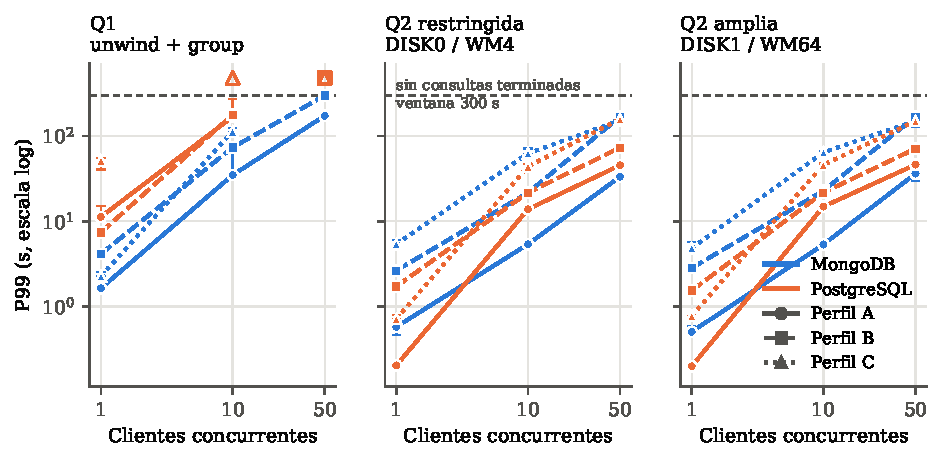
\includegraphics[width=\linewidth]{p99_vs_concurrencia.pdf}
\caption{P99 frente a concurrencia (ejes logarítmicos), mediana de 3 repeticiones con el rango
mínimo--máximo. Color: motor; marcador y trazo: perfil. Los marcadores huecos sobre la línea de
300\,s son celdas en las que ninguna consulta terminó dentro de la ventana (latencia censurada).}
\label{fig:p99}
\end{figure}

\noindent La figura~\ref{fig:p99} muestra que el P99 crece casi en proporción a la concurrencia en
cuanto la CPU se satura. Pasar de 1 a 10 clientes multiplica el P99 de Q1 en MongoDB por
$\sim$21 en A y por $\sim$50 en C. En Q2 la pendiente de PostgreSQL es más fuerte: parte de
0.2\,s, pero con 10 clientes ya compite con MongoDB porque cada consulta usa hasta 3 procesos y
satura la cuota con un solo cliente.

\begin{figure}[H]\centering
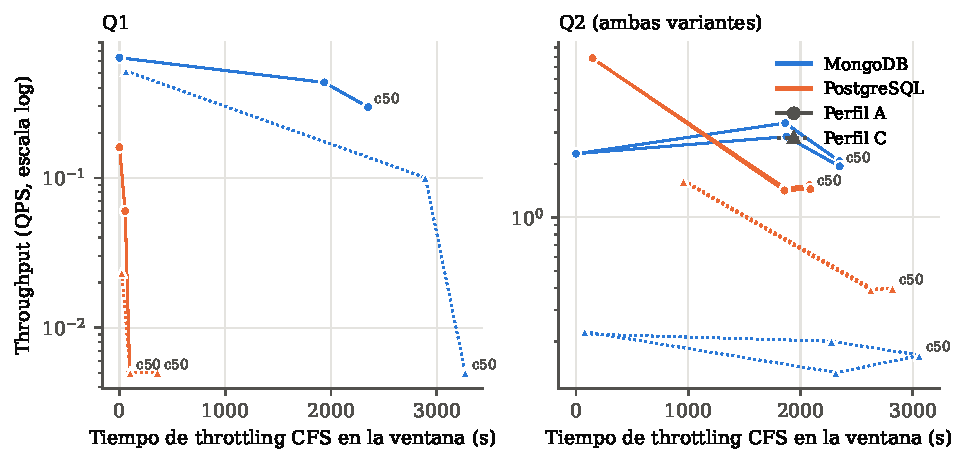
\includegraphics[width=\linewidth]{throttling_vs_qps.pdf}
\caption{Throttling CFS acumulado en la ventana frente a throughput (mediana por celda). Cada
trazo recorre las concurrencias 1, 10 y 50 de un motor y un perfil; el final del trazo está
etiquetado. Las celdas con 0\,QPS se dibujan en el borde inferior.}
\label{fig:throttling}
\end{figure}

\noindent En la figura~\ref{fig:throttling}, más concurrencia aumenta el throttling sin aumentar
el throughput: la cuota ya está agotada, y el trabajo extra solo se convierte en cola. En Q1 en A y
C, el throttling de PostgreSQL es bajo (menos de 400\,s) incluso cuando no termina ninguna
consulta: el cuello de botella no es la CPU sino la escritura y lectura de los archivos temporales
del ordenamiento. En B, PostgreSQL Q1 sí se acerca a su cuota (558 de 600\,CPU-s con 50 clientes)
y acumula 780--1\,264\,s de throttling. B corrió solo en su equipo, mientras que A y C compartían el
disco donde volcaban sus temporales; es consistente con que el disco compartido frenara a
PostgreSQL en la ronda~1, aunque con un solo equipo para B no se puede separar del efecto del
hardware.

\begin{figure}[H]\centering
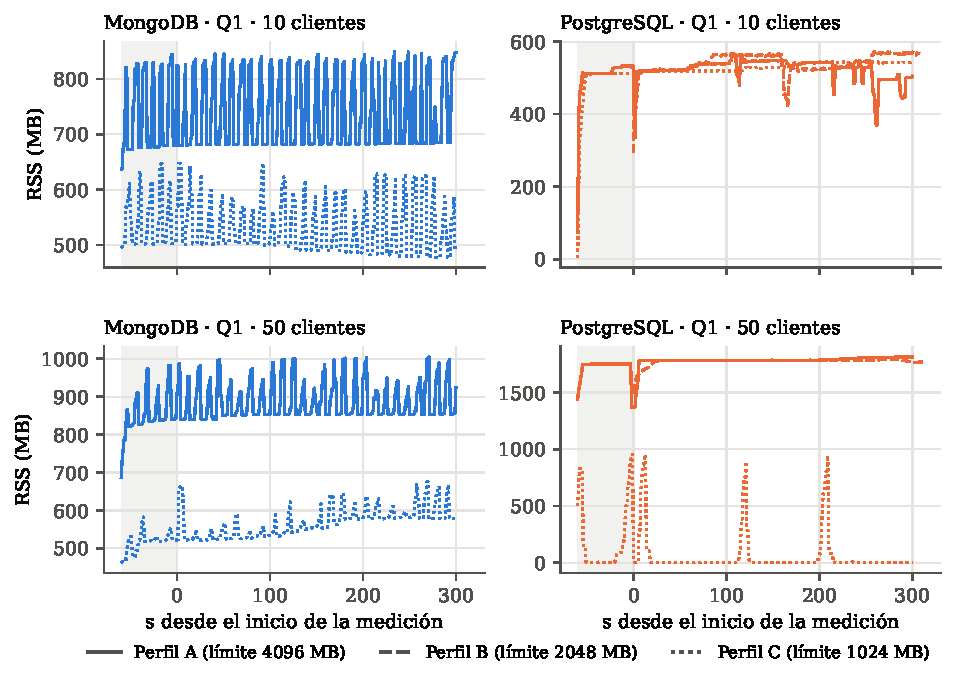
\includegraphics[width=\linewidth]{curva_rss_q1.pdf}
\caption{Curva de RSS del contenedor durante Q1 (repetición 1), cada 1\,s desde Prometheus o
desde la cgroup. La banda gris es el warmup. MongoDB en B no tiene curva por la falta de serie descrita en
la sección~\ref{sec:validez}.}
\label{fig:rss}
\end{figure}

\noindent La figura~\ref{fig:rss} muestra el patrón de memoria de cada motor. MongoDB oscila en
dientes de sierra, del orden de 150\,MB por consulta, por encima de su caché WiredTiger, y nunca se
acerca al límite. En PostgreSQL con 1\,GB y 50 clientes el RSS sube hasta $\sim$950\,MB y cae a
cero en cada \texttt{oom\_kill}: el \emph{postmaster} reinicia los procesos y entra en
\emph{recovery} varias veces dentro de la misma ventana. Con 4\,GB, el RSS de PostgreSQL se
estabiliza en $\sim$1.8\,GB; con 2\,GB (B) llega a la misma cifra, a 250\,MB del límite, sin
llegar al OOM.

% =============================================================================
\section{Planes de ejecución}
\label{sec:planes}
Los 18 planes (2 motores $\times$ 3 consultas $\times$ 3 perfiles) están en
\texttt{results/explain/}: \texttt{explain("executionStats")} en MongoDB y
\texttt{EXPLAIN (ANALYZE, BUFFERS)} en PostgreSQL, capturados con un solo cliente.

\begin{table}[H]\centering\small
\caption{Resumen de los planes en el perfil A (los perfiles B y C tienen la misma forma).}
\label{tab:planes}
\begin{tabularx}{\linewidth}{llX}
\toprule
Consulta & Motor & Plan y memoria \\
\midrule
Q1 & MongoDB & \texttt{COLLSCAN} de 500\,000 documentos $\rightarrow$ \texttt{\$unwind} (1\,500\,160) $\rightarrow$ \texttt{\$match} (974\,583) $\rightarrow$ \texttt{\$group} (180 grupos). Memoria de agrupación: 128\,KB. \texttt{usedDisk: false}, 0 spills. 2.2\,s en A, 2.3\,s en C. \\
\addlinespace
Q1 & PostgreSQL & \texttt{Parallel Seq Scan} (2 workers) $\rightarrow$ \texttt{Sort} de filas completas (ancho estimado 1\,304\,B) con \textbf{external merge}: 192 + 235 + 226\,MB en disco $\rightarrow$ \texttt{Gather Merge} $\rightarrow$ \texttt{jsonb\_array\_elements} $\rightarrow$ \texttt{Incremental Sort} (external merge) $\rightarrow$ \texttt{GroupAggregate}. \textbf{Temp: 187\,865 bloques escritos} ($\approx$1.5\,GB). El planificador estima 16.5 millones de grupos frente a 180 reales. 10.0\,s en A, 20.6\,s en C. \\
\addlinespace
Q2 & MongoDB & \texttt{IXSCAN} sobre \texttt{idx\_cerrado\_en} (250\,141 claves) $\rightarrow$ \texttt{FETCH} y filtro (212\,641) $\rightarrow$ \texttt{SORT} top-$k$ con límite 1000 (\texttt{memLimit} 100\,MB, pico 1.09\,MB) $\rightarrow$ \texttt{PROJECTION}. Sin disco con \texttt{allowDiskUse} false ni true. 0.45\,s en A, 5.5\,s en C. \\
\addlinespace
Q2 & PostgreSQL & \texttt{Parallel Seq Scan} (2 workers, 500\,000 filas; no usa el índice de fecha porque el filtro conserva $\sim$42\,\% de la tabla) $\rightarrow$ \texttt{Sort} \textbf{top-N heapsort} de 272\,KB por proceso $\rightarrow$ \texttt{Gather Merge} $\rightarrow$ \texttt{Limit}. Igual con \texttt{work\_mem} de 4\,MB y de 64\,MB. 0.12\,s en A, 0.88\,s en C. \\
\bottomrule
\end{tabularx}
\end{table}

\noindent Los planes respaldan los cuellos de botella medidos:
\begin{itemize}
  \item \textbf{Q1 en PostgreSQL}: con el \texttt{work\_mem} por defecto, un ordenamiento de
        $\sim$650\,MB obliga a usar disco. El volumen temporal de una consulta en el plan
        ($\approx$1.5\,GB) es coherente con lo medido: 42.5\,GB en una ventana de A con un cliente, que
        terminó 48 consultas ($\approx$0.9\,GB por consulta, más las que quedaron a medias). La
        mala estimación de grupos lleva al planificador a ordenar en lugar de usar un
        \texttt{HashAggregate} de 180 grupos.
  \item \textbf{Q1 en MongoDB}: el pipeline procesa en flujo y su agrupación ocupa kilobytes, así
        que solo lo limita la CPU, como confirma el throttling (sección~\ref{sec:interpretacion}).
  \item \textbf{Q2}: el Top-1000 nunca necesita más de $\sim$1\,MB en ningún motor, así que las
        variantes \texttt{allowDiskUse} y \texttt{work\_mem} no cambian el plan ni el resultado.
        La especificación pide reportar las variantes con y sin spill; en Q2 ambas resultan sin spill,
        y el contraste con volcado a disco lo aporta Q1.
\end{itemize}

% =============================================================================
\section{Interpretación: memoria, volcado a disco y throttling}
\label{sec:interpretacion}

\subsection*{M1. ¿Cómo cambian P95 y P99 al limitar CPU y memoria?}
\begin{itemize}
  \item \textbf{Con un cliente} el efecto es moderado cuando la consulta usa un solo núcleo
        (MongoDB Q1: P99 de 1.6\,s en A a 2.3\,s en C, $\times$1.4) y fuerte cuando la consulta
        usa varios núcleos o disco. MongoDB Q2 sube de 0.58 a 5.4\,s ($\times$9.3) y PostgreSQL Q1
        de 11.3 a 51.9\,s ($\times$4.6), porque en C sus workers paralelos y su I/O temporal
        compiten por un solo núcleo.
  \item \textbf{Con concurrencia} el P99 lo dominan la cola y el throttling. Con 10 clientes la
        cuota se agota en los tres perfiles (A: 1\,200\,CPU-s de 1\,200 posibles; B: $\sim$580
        de 600; C: 300 de 300) y el P99 crece en proporción al número de clientes por núcleo.
  \item \textbf{P95 y P99 quedan casi pegados} cuando el sistema está saturado, como en MongoDB Q1
        con 10 clientes en C (P95 113.2\,s, P99 113.3\,s): todas las consultas esperan lo mismo y
        la cola de la distribución desaparece. La degradación se ve también en el P50.
  \item \textbf{El límite de memoria cambia el resultado}, y no solo la latencia, en PostgreSQL Q1:
        con 1\,GB y 50 clientes el contenedor muere (28 \texttt{oom\_kill} en 3 repeticiones).
  \item \textbf{En B} el efecto con concurrencia es intermedio entre A y C: el P99 de MongoDB Q1
        con 10 clientes es 73.6\,s (34.9 en A, 113.3 en C) y el de PostgreSQL Q2 con 10 clientes,
        21.7\,s (13.9 en A, 44.1 en C). Con un cliente B no es intermedio porque su
        equipo tiene núcleos más lentos; la comparación que aísla el efecto del límite es A frente
        a C, medidos en el mismo hardware.
\end{itemize}

\subsection*{M2. ¿Qué motor gestiona mejor los buffers antes de spill u OOM?}
\begin{itemize}
  \item \textbf{En la agregación con desanidado (Q1), MongoDB.} Agrupa en flujo con un estado de
        $\sim$128\,KB, nunca vuelca a disco y no tuvo ningún OOM en ningún perfil. Con 1\,GB y 50
        clientes falla por tiempo (CPU), no por memoria.
  \item \textbf{PostgreSQL vuelca a disco en todas las corridas de Q1} que llegan a ejecutar
        consultas: el ordenamiento de filas completas no cabe en 4\,MB de \texttt{work\_mem}.
        Escribe 6.7--7.1\,GB por ventana en C, 13.5--47.6\,GB en B y 22.9--42.5\,GB en A, y con
        50 backends en 1\,GB termina en OOM: cada backend y sus workers reservan memoria propia
        para ordenar y descomprimir (\emph{detoast}) el JSONB, y la suma rebasa el límite.
  \item \textbf{En el Top-K (Q2) los dos gestionan bien el buffer.} Ambos usan un ordenamiento
        top-$k$ acotado (1.09\,MB en MongoDB, 272\,KB por proceso en PostgreSQL), muy por debajo
        de \texttt{memLimit} (100\,MB) y de \texttt{work\_mem} (4\,MB). Ninguna de las 108
        corridas de Q2 (54 por motor, en los tres perfiles) presentó spill u OOM.
\end{itemize}

\subsection*{M3. Huella de CPU y memoria por cada 1\,000 documentos}
Se definen como:
\[
\text{CPU-s}/1000 = \frac{\text{CPU-s de la ventana}}{\text{consultas terminadas}\times 500\,000}\times 1000,
\qquad
\text{MB}/1000 = \frac{\text{RSS máximo}}{500\,000}\times 1000 .
\]
El denominador son los 500\,000 documentos de la colección que evalúa cada consulta. Se usa la
concurrencia 1, donde el costo por consulta no incluye tiempo de cola. Los CPU-s salen de
\texttt{container\_cpu\_usage\_seconds\_total} (Prometheus) o de \texttt{usage\_usec} de la
cgroup (\texttt{results/series/}).

\begin{table}[H]\centering\small
\caption{M3 con un cliente: CPU-s y MB de RSS por cada 1\,000 documentos (mediana de 3
repeticiones). $^\dagger$ Estimado: sin serie de CPU para esa celda, se usa la cuota del
perfil o el consumo de la misma celda en A, el menor de los dos.}
\label{tab:m3}
\begin{tabular}{llrrrr}
\toprule
 & & \multicolumn{2}{c}{Perfil A} & \multicolumn{2}{c}{Perfil C} \\
\cmidrule(lr){3-4} \cmidrule(lr){5-6}
Motor & Query & CPU-s & MB & CPU-s & MB \\
\midrule
MongoDB & Q1 & 0.0034 & 1.587 & 0.0039 & 1.258 \\
MongoDB & Q2\_DISK0 & 0.0010 & 2.022 & 0.0091 & 1.478 \\
MongoDB & Q2\_DISK1 & 0.0009 & 2.000 & 0.0088 & 1.440 \\
\midrule
PostgreSQL & Q1 & 0.0091 & 0.204 & 0.0128 & 0.203 \\
PostgreSQL & Q2\_WM4 & 0.0010 & 0.028 & 0.0012 & 0.032 \\
PostgreSQL & Q2\_WM64 & 0.0010 & 0.029 & 0.0013 & 0.032 \\
\bottomrule
\end{tabular}

\end{table}

\begin{itemize}
  \item \textbf{CPU}: en Q1, MongoDB gasta $\sim$0.0034\,CPU-s por 1\,000 documentos y
        PostgreSQL $\sim$0.0091 en A, 2.7 veces más, a pesar de usar menos CPU en total:
        PostgreSQL pasa la mayor parte del tiempo esperando disco y termina menos consultas. En
        Q2 los dos están en $\sim$0.001 en A; en C, MongoDB sube a 0.009 (el \texttt{FETCH} de
        250\,141 documentos con un núcleo) y PostgreSQL se mantiene en 0.0012. En B, MongoDB Q2
        queda entre ambos (0.0039) y PostgreSQL Q2 por encima de los dos (0.0028): con 2~CPU sus
        3 procesos paralelos agotan la cuota con un solo cliente sin terminar más consultas. El
        valor de MongoDB Q1 en B (0.0056) es una cota superior estimada.
  \item \textbf{Memoria}: el RSS de MongoDB (1.3--2.0\,MB por 1\,000 documentos) incluye su caché
        WiredTiger, que vive en memoria anónima. El de PostgreSQL (0.03--0.2\,MB) no incluye
        \texttt{shared\_buffers}, que es memoria compartida. Las cifras de memoria no son
        un costo marginal por consulta, sino la huella del proceso con el límite dado.
\end{itemize}

\subsection*{Throttling de cgroups}
Con 10 o más clientes ambos motores consumen casi exactamente su cuota de CPU (1\,200\,CPU-s en A,
600 en B y 300 en C por ventana), y el throttling acumulado va de 1\,850 a 3\,280\,s en A y C y de
1\,480 a 1\,820\,s en B. Es más que la ventana porque se suma por cada CPU en la que había hilos
esperando. La excepción es PostgreSQL Q1, con menos de 400\,s de throttling en A y C: no
espera CPU sino disco temporal. En B llega a 780--1\,264\,s (sección~\ref{sec:graficas}).
PostgreSQL Q2 sufre throttling incluso con un cliente (137\,s en A, 642 en B, 958 en C), porque
su consulta paralela usa 3 procesos y con 2 o 1 CPU satura la cuota sola.

\subsection*{Respuestas a las preguntas del revisor}
\begin{enumerate}
  \item \textbf{¿El baseline es comparable?} Sí, en dataset y consultas: el mismo NDJSON
        (sha256 verificado), la misma validación y resultados equivalentes en ambos motores
        (sección~\ref{sec:metodo}). En hardware, A y C comparten equipo y B no
        (sección~\ref{sec:validez}).
  \item \textbf{¿P50/P95/P99 o promedios?} Percentiles sobre las latencias individuales de cada
        corrida (tablas~\ref{tab:resA}--\ref{tab:resC}); las latencias crudas están en
        \texttt{results/raw/}.
  \item \textbf{¿Hubo throttling CFS? ¿Cuántos segundos?} Sí, en todas las celdas con 10 y 50
        clientes, y con 1 cliente en C y en PostgreSQL Q2. Hasta 3\,280\,s por ventana (columna ``Throttled'' y
        figura~\ref{fig:throttling}).
  \item \textbf{¿Spill u OOM? ¿En qué perfil y concurrencia?} Spill en PostgreSQL Q1 en todos los
        perfiles y concurrencias; OOM en PostgreSQL Q1, perfil C, 50 clientes. MongoDB y Q2 sin
        spill (tabla~\ref{tab:spill}, evidencia en \texttt{results/evidencia\_spill\_oom/}).
  \item \textbf{¿Cuántas repeticiones y cómo se resumen?} 3 por celda, mediana con rango
        mínimo--máximo.
  \item \textbf{¿El plan respalda el cuello de botella?} Sí: el external merge de PostgreSQL Q1
        explica su spill y su bajo uso de CPU; el pipeline en flujo de MongoDB explica que solo lo
        limite la CPU; el top-$k$ de ambos explica la ausencia de spill en Q2
        (sección~\ref{sec:planes}).
\end{enumerate}

% =============================================================================
\section{Recomendaciones técnicas para despliegues documentales en la nube}
\label{sec:recomendaciones}
\begin{enumerate}
  \item \textbf{Dimensionar la CPU por el P99, no por el promedio.} Con cuotas CFS estrictas, el
        P99 crece en proporción a los clientes por núcleo una vez agotada la cuota. Conviene
        vigilar \texttt{throttled\_usec} (o \texttt{container\_cpu\_cfs\_throttled\_seconds\_total})
        como señal de saturación junto al P99. En cargas sensibles a latencia, valorar no imponer
        límite de CPU o reservar núcleos (\emph{requests} cercanos al límite).
  \item \textbf{Limitar la concurrencia en PostgreSQL con un \emph{pooler}} (PgBouncer o el de la
        aplicación). La memoria de PostgreSQL crece con el número de backends y sus workers; con
        contenedores pequeños, el OOM llega por concurrencia antes que por tamaño de datos.
        Ajustar \texttt{max\_parallel\_workers\_per\_gather} al número de CPU del contenedor.
  \item \textbf{Revisar \texttt{work\_mem} y el plan de las agregaciones JSONB con desanidado.}
        La estimación por defecto de \texttt{jsonb\_array\_elements} lleva a ordenar filas
        completas a disco. Opciones: subir \texttt{work\_mem} por sesión solo para esas
        consultas (con el límite del contenedor en mente: $\text{work\_mem}\times$ procesos),
        reescribir la consulta para proyectar las claves antes de agrupar, o normalizar el arreglo
        en una tabla propia si la agregación es frecuente.
  \item \textbf{MongoDB para agregaciones en flujo con memoria acotada.} Su pipeline mantuvo un
        estado de kilobytes y nunca hizo spill; su límite es la CPU: escalar núcleos mejora el
        throughput con concurrencia, no la latencia de una consulta aislada (un hilo por consulta).
  \item \textbf{Sin swap y con margen de memoria.} Con \texttt{memory.swap.max = 0} la presión de
        memoria se manifiesta como OOM visible y no como latencia oculta; dejar margen para la
        caché de WiredTiger o los \texttt{shared\_buffers} más la memoria por conexión.
  \item \textbf{Índices y Top-K.} Un Top-K con \texttt{LIMIT} se resuelve con un ordenamiento
        acotado en ambos motores; no es necesario indexar el campo de orden para evitar el spill.
        Sí conviene un índice selectivo para el filtro: MongoDB lo usa (250\,141 claves); a
        PostgreSQL no le compensa con una selectividad del 42\,\%.
\end{enumerate}

% =============================================================================
\section*{Amenazas a la validez}
\label{sec:validez}
\addcontentsline{toc}{section}{Amenazas a la validez}
\begin{itemize}
  \item \textbf{Equipos distintos.} B se midió en otro equipo (i5-1135G7 de 11.ª generación frente
        al i5-13420H de 13.ª), así que su comparación con A y C mezcla el efecto del límite con el
        del hardware. Se nota con un cliente, donde B resulta a veces más lento que C. La
        comparación entre motores dentro de cada perfil sí es homogénea.
  \item \textbf{Perfiles en paralelo.} A y C compartieron equipo; sus límites no se solapan
        (5 de 12 hilos, 5 de 7.6\,GB), pero comparten caché L3, memoria y disco. El disco
        compartido afecta sobre todo a PostgreSQL Q1, que escribe decenas de GB temporales por
        ventana; B, que corrió solo, muestra más uso de CPU en esa celda.
  \item \textbf{Telemetría en el equipo de B.} En ese equipo, cAdvisor no exponía las
        métricas por contenedor, así que el programa de medición pasó a leer la CPU y el RSS
        directamente de la cgroup de cada contenedor, con el mismo significado. Las 9 corridas
        de MongoDB Q1, las primeras de B, se hicieron antes de ese cambio y no tienen serie de
        CPU ni de RSS: su M3 de CPU es una cota ($^\dagger$ en la tabla~\ref{tab:m3}), mientras
        que su throttling y su RSS máximo sí se midieron.
  \item \textbf{Ventana censurada.} Cuando una consulta dura más que la ventana, la latencia no se
        registra y el P99 subestima la cola; esas celdas se marcan \texttt{error} con 0\,QPS. Los
        CPU-s de la ventana incluyen el trabajo de consultas cortadas, lo que encarece M3 en las
        celdas saturadas (por eso M3 usa 1 cliente).
  \item \textbf{Telemetría propia.} El \emph{healthcheck} de MongoDB (\texttt{mongosh} cada 5\,s)
        corre dentro de la cgroup y consume algo de CPU en todos los perfiles.
  \item \textbf{Virtualización.} WSL2 añade una capa de virtualización; el flush de caché vacía la
        page cache del kernel de la VM, no la del host Windows.
  \item \textbf{Tres repeticiones} dan un rango, no un intervalo de confianza.
\end{itemize}

% =============================================================================
\appendix
\section{Reproducción y artefactos}
\begin{itemize}
  \item Repositorio: \url{https://github.com/lsprz2773/BDN-Exp}. Preparación:
        \texttt{scripts/setup\_env.sh <perfil>}; ronda: \texttt{scripts/run\_benchmarks.sh
        --profile <P> --round <N>} (con \texttt{--parties} y \texttt{--session} para medir dos
        perfiles en paralelo). Las instrucciones completas están en el \texttt{README.md}.
  \item Mediciones: \texttt{results/csv/mediciones\_ronda1.csv} y
        \texttt{mediciones\_ronda2.csv}, con las 14 columnas de la especificación y el mismo encabezado.
  \item Latencias crudas, series de RSS/CPU, planes, entorno y evidencia de spill/OOM en
        \texttt{results/raw}, \texttt{results/series}, \texttt{results/explain},
        \texttt{results/entorno} y \texttt{results/evidencia\_spill\_oom}.
  \item Tablas y figuras de este reporte: \texttt{scripts/analyze\_results.py}.
\end{itemize}

\noindent Ejemplo de fila del CSV (perfil C, PostgreSQL Q1, 1 cliente):
\begin{lstlisting}
timestamp_epoch,engine,profile,query_id,concurrency,run_number,throughput_qps,latency_p50_ms,latency_p95_ms,latency_p99_ms,cpu_throttled_seconds,max_rss_mb,disk_spill,status
1793571192,postgresql,PROFILE_C_SEVERE,Q1,1,1,0.0333,27021.55,38973.8,40516.35,25.767,101.4,true,spill
\end{lstlisting}

\end{document}
